%  LaTeX support: latex@mdpi.com
%  In case you need support, please attach all files that are necessary for compiling as well as the log file, and specify the details of your LaTeX setup (which operating system and LaTeX version / tools you are using).

%=================================================================
\documentclass[ijerph,article,submit,moreauthors,pdftex]{mdpi}

% If you would like to post an early version of this manuscript as a preprint, you may use preprint as the journal and change 'submit' to 'accept'. The document class line would be, e.g., \documentclass[preprints,article,accept,moreauthors,pdftex]{mdpi}. This is especially recommended for submission to arXiv, where line numbers should be removed before posting. For preprints.org, the editorial staff will make this change immediately prior to posting.

%% Some pieces required from the pandoc template
\setlist[itemize]{leftmargin=*,labelsep=5.8mm}
\setlist[enumerate]{leftmargin=*,labelsep=4.9mm}


%--------------------
% Class Options:
%--------------------
%----------
% journal
%----------
% Choose between the following MDPI journals:
% acoustics, actuators, addictions, admsci, aerospace, agriculture, agriengineering, agronomy, algorithms, animals, antibiotics, antibodies, antioxidants, applsci, arts, asc, asi, atmosphere, atoms, axioms, batteries, bdcc, behavsci , beverages, bioengineering, biology, biomedicines, biomimetics, biomolecules, biosensors, brainsci , buildings, cancers, carbon , catalysts, cells, ceramics, challenges, chemengineering, chemistry, chemosensors, children, cleantechnol, climate, clockssleep, cmd, coatings, colloids, computation, computers, condensedmatter, cosmetics, cryptography, crystals, dairy, data, dentistry, designs , diagnostics, diseases, diversity, drones, econometrics, economies, education, electrochem, electronics, energies, entropy, environments, epigenomes, est, fermentation, fibers, fire, fishes, fluids, foods, forecasting, forests, fractalfract, futureinternet, futurephys, galaxies, games, gastrointestdisord, gels, genealogy, genes, geohazards, geosciences, geriatrics, hazardousmatters, healthcare, heritage, highthroughput, horticulturae, humanities, hydrology, ijerph, ijfs, ijgi, ijms, ijns, ijtpp, informatics, information, infrastructures, inorganics, insects, instruments, inventions, iot, j, jcdd, jcm, jcp, jcs, jdb, jfb, jfmk, jimaging, jintelligence, jlpea, jmmp, jmse, jnt, jof, joitmc, jpm, jrfm, jsan, land, languages, laws, life, literature, logistics, lubricants, machines, magnetochemistry, make, marinedrugs, materials, mathematics, mca, medicina, medicines, medsci, membranes, metabolites, metals, microarrays, micromachines, microorganisms, minerals, modelling, molbank, molecules, mps, mti, nanomaterials, ncrna, neuroglia, nitrogen, notspecified, nutrients, ohbm, particles, pathogens, pharmaceuticals, pharmaceutics, pharmacy, philosophies, photonics, physics, plants, plasma, polymers, polysaccharides, preprints , proceedings, processes, proteomes, psych, publications, quantumrep, quaternary, qubs, reactions, recycling, religions, remotesensing, reports, resources, risks, robotics, safety, sci, scipharm, sensors, separations, sexes, signals, sinusitis, smartcities, sna, societies, socsci, soilsystems, sports, standards, stats, surfaces, surgeries, sustainability, symmetry, systems, technologies, test, toxics, toxins, tropicalmed, universe, urbansci, vaccines, vehicles, vetsci, vibration, viruses, vision, water, wem, wevj

%---------
% article
%---------
% The default type of manuscript is "article", but can be replaced by:
% abstract, addendum, article, benchmark, book, bookreview, briefreport, casereport, changes, comment, commentary, communication, conceptpaper, conferenceproceedings, correction, conferencereport, expressionofconcern, extendedabstract, meetingreport, creative, datadescriptor, discussion, editorial, essay, erratum, hypothesis, interestingimages, letter, meetingreport, newbookreceived, obituary, opinion, projectreport, reply, retraction, review, perspective, protocol, shortnote, supfile, technicalnote, viewpoint
% supfile = supplementary materials

%----------
% submit
%----------
% The class option "submit" will be changed to "accept" by the Editorial Office when the paper is accepted. This will only make changes to the frontpage (e.g., the logo of the journal will get visible), the headings, and the copyright information. Also, line numbering will be removed. Journal info and pagination for accepted papers will also be assigned by the Editorial Office.

%------------------
% moreauthors
%------------------
% If there is only one author the class option oneauthor should be used. Otherwise use the class option moreauthors.

%---------
% pdftex
%---------
% The option pdftex is for use with pdfLaTeX. If eps figures are used, remove the option pdftex and use LaTeX and dvi2pdf.

%=================================================================
\firstpage{1}
\makeatletter
\setcounter{page}{\@firstpage}
\makeatother
\pubvolume{xx}
\issuenum{1}
\articlenumber{5}
\pubyear{2019}
\copyrightyear{2019}
%\externaleditor{Academic Editor: name}
\history{Received: date; Accepted: date; Published: date}
\updates{yes} % If there is an update available, un-comment this line

%% MDPI internal command: uncomment if new journal that already uses continuous page numbers
%\continuouspages{yes}

%------------------------------------------------------------------
% The following line should be uncommented if the LaTeX file is uploaded to arXiv.org
%\pdfoutput=1

%=================================================================
% Add packages and commands here. The following packages are loaded in our class file: fontenc, calc, indentfirst, fancyhdr, graphicx, lastpage, ifthen, lineno, float, amsmath, setspace, enumitem, mathpazo, booktabs, titlesec, etoolbox, amsthm, hyphenat, natbib, hyperref, footmisc, geometry, caption, url, mdframed, tabto, soul, multirow, microtype, tikz

%=================================================================
%% Please use the following mathematics environments: Theorem, Lemma, Corollary, Proposition, Characterization, Property, Problem, Example, ExamplesandDefinitions, Hypothesis, Remark, Definition
%% For proofs, please use the proof environment (the amsthm package is loaded by the MDPI class).

%=================================================================
% Full title of the paper (Capitalized)
\Title{Beyond proximity: utility-based access from location-based services data.}

% Authors, for the paper (add full first names)
\Author{Gregory S. Macfarlane$^{1, *}$, Emma Stucki$^{1}$, Alisha Redelfs$^{2}$, Lori Spruance$^{2}$}

% Authors, for metadata in PDF
\AuthorNames{Gregory S. Macfarlane, Emma Stucki, Alisha Redelfs, Lori Spruance}

% Affiliations / Addresses (Add [1] after \address if there is only one affiliation.)
\address{%
$^{1}$ \quad Brigham Young University, Civil and Construction Engineering Department; \\
$^{2}$ \quad Brigham Young University, Public Health Department; \\
}
% Contact information of the corresponding author
\corres{Correspondence: \href{mailto:gregmacfarlane@byu.edu}{\nolinkurl{gregmacfarlane@byu.edu}}; Tel.: +1.801.422.8505}

% Current address and/or shared authorship








% The commands \thirdnote{} till \eighthnote{} are available for further notes

% Simple summary
\simplesumm{Proximity to community resources is often used as a benchmark in spatial
public health analyses, but a measure that incorporates observed preferences
leads to different policy interventions.}

% Abstract (Do not insert blank lines, i.e. \\)
\abstract{Understanding who in a community has access to its resources -- parks, libraries, grocery stores, etc. -- has profound equity implications, but typical methods to understand access to these resources are limited. Travel time buffers require researchers to assert mode of access as well as an arbitrary distance threshold; further, these methods do not distinguish between destination quality attributes in an effective way. In this research, we present a methodology to develop utility-based accessibility measures for parks, libraries, and grocery stores in Utah County, Utah. The method relies on passive location-based services data to model destination choice to these community resources; the destination choice model utility functions in turn allow us to develop a picture of regional access that is sensitive to: the quality and size of the destination resource; continuous (non-binary) travel impedance by multiple modes; and the sociodemographic attributes of the traveler. We then use this measure to explore equity in access to the specified community resources across income level in Utah County: the results reveal a discrepancy between which neighborhoods might be targeted for intervention using space-based analysis.}

% Keywords
\keyword{Accessibility; Spatial analysis}

% The fields PACS, MSC, and JEL may be left empty or commented out if not applicable
%\PACS{J0101}
%\MSC{}
%\JEL{}

%%%%%%%%%%%%%%%%%%%%%%%%%%%%%%%%%%%%%%%%%%
% Only for the journal Diversity
%\LSID{\url{http://}}

%%%%%%%%%%%%%%%%%%%%%%%%%%%%%%%%%%%%%%%%%%
% Only for the journal Applied Sciences:
%\featuredapplication{Authors are encouraged to provide a concise description of the specific application or a potential application of the work. This section is not mandatory.}
%%%%%%%%%%%%%%%%%%%%%%%%%%%%%%%%%%%%%%%%%%

%%%%%%%%%%%%%%%%%%%%%%%%%%%%%%%%%%%%%%%%%%
% Only for the journal Data:
%\dataset{DOI number or link to the deposited data set in cases where the data set is published or set to be published separately. If the data set is submitted and will be published as a supplement to this paper in the journal Data, this field will be filled by the editors of the journal. In this case, please make sure to submit the data set as a supplement when entering your manuscript into our manuscript editorial system.}

%\datasetlicense{license under which the data set is made available (CC0, CC-BY, CC-BY-SA, CC-BY-NC, etc.)}

%%%%%%%%%%%%%%%%%%%%%%%%%%%%%%%%%%%%%%%%%%
% Only for the journal Toxins
%\keycontribution{The breakthroughs or highlights of the manuscript. Authors can write one or two sentences to describe the most important part of the paper.}

%\setcounter{secnumdepth}{4}
%%%%%%%%%%%%%%%%%%%%%%%%%%%%%%%%%%%%%%%%%%


% tightlist command for lists without linebreak
\providecommand{\tightlist}{%
  \setlength{\itemsep}{0pt}\setlength{\parskip}{0pt}}

% From pandoc table feature
\usepackage{longtable,booktabs,array}
\usepackage{calc} % for calculating minipage widths
% Correct order of tables after \paragraph or \subparagraph
\usepackage{etoolbox}
\makeatletter
\patchcmd\longtable{\par}{\if@noskipsec\mbox{}\fi\par}{}{}
\makeatother
% Allow footnotes in longtable head/foot
\IfFileExists{footnotehyper.sty}{\usepackage{footnotehyper}}{\usepackage{footnote}}
\makesavenoteenv{longtable}


\usepackage{hyperref}
\usepackage[utf8]{inputenc}
\def\tightlist{}
\usepackage{booktabs}
\usepackage{longtable}
\usepackage{array}
\usepackage{multirow}
\usepackage{wrapfig}
\usepackage{float}
\usepackage{colortbl}
\usepackage{pdflscape}
\usepackage{tabu}
\usepackage{threeparttable}
\usepackage{threeparttablex}
\usepackage[normalem]{ulem}
\usepackage{makecell}
\usepackage{xcolor}

\begin{document}


%%%%%%%%%%%%%%%%%%%%%%%%%%%%%%%%%%%%%%%%%%

\hypertarget{intro}{%
\section{Introduction}\label{intro}}

Communities provide important resources to the people who live in them. These
resources might include physical and economic resources
--- shared open space, libraries, commercial establishments, etc. --- as well as less identifiable resources
including a sense of membership and other forms of social capital
\citep{lochner1999}. Indeed, access to these resources is a primary reason why
communities exist \citep{muth1971}, as well as a long-motivating objective in
transportation infrastructure planning \citep{hansen1959}.

Given the importance of these community resources, it is not surprising that
so much scholarly attention has been paid to examining the spatial and
socioeconomic variation in access to them \citep{handy1997, witten2003}. What
is surprising is the simplistic and arbitrary definition of many
quantitative resource accessibility measures, in spite of the widespread
availability of geographical information systems (GIS) software \citep{logan2019} and
an understanding that proximity to a resource is not the only consideration
in its use \citep{dong2006}. Individuals do not always shop at the nearest grocery
store, nor do they necessarily perceive an 11-minute walk to a park as
meaningfully different from a 9-minute walk. A measure of access that can
incorporate travel impedance by multiple transportation modes alongside
qualitative attributes of the resources in question would provide a better
theoretical comparison to what people experience and observe in their own
communities. This measure in turn may result in a different understanding
of which groups have or do not have good access --- and therefore in different
policy interventions to resolve the access gap --- than more traditionally used
measures \citep{logan2019, macfarlane2020}.

In this paper, we develop utility-based access measures to parks, grocery stores, and
libraries in Utah County, Utah. These measures are based in econometric choice
theory relating continuous multimodal travel impedance to attributes of the
resource. The utility preferences are estimated on location-based services data
obtained from a third-party commercial data aggregator. We then use the model
estimates to construct a composite accessibility measure and examine potential
discrepancies between this measure and a more common travel-time buffer
measurement.

The paper begins with a discussion of previous findings relating access to
community resources with social, health, and equity benefits. We then describe
the methodology employed in this research, which makes use of novel third-party
mobile device. A results section describes both the estimated choice models and
a comparative analysis; the paper closes with a discussion of several
limitations of the approach as well as associated opportunities for future research.

\hypertarget{lit-review}{%
\section{Literature}\label{lit-review}}

In this study, we have chosen to focus on three specific community resources
that have robust histories of accessibility and spatial analysis: parks, grocery
stores, and libraries. This section first discusses research developing and
classifying various accessibility measures, followed by a discussion of previous
attempts to measure access to the resources selected for this analysis.

\hypertarget{developing-access-measures}{%
\subsection{Developing Access Measures}\label{developing-access-measures}}

Accessibility is easily defined as the ability to reach useful destinations \citep{handy1997},
but this ease in definition belies a wide array of potential quantitative
descriptions. \citet{dong2006} present a helpful hierarchy of access measures, which we
briefly summarize here.

Among the simplest measures of access is a so-called isochrone or buffer measure, which
considers whether a person at position \(i\) traveling to a potential destination
\(j\) is within a particular travel time threshold \(t^*\). Using this measure, a
person has access to the resource if \(t_{ij} < t^*\). Sometimes it is
possible to access multiple resources within this threshold, in which case a
a cumulative opportunities measure can be defined as
\begin{equation}
  A_i^{\mathrm{isochrone}} = \sum_{j \in J} \delta_{ij}, 
  \mathrm{\ where\ } \delta_{ij} = 
  \begin{cases}
    1, & \text{for } t_{ij} \leq t^*\\
    0, & \text{for } t_{ij} > t^*
  \end{cases} 
  \label{eq:isochrone}
\end{equation}
Variations of this measure include elements like ``number of grocery stores
within 10 minutes'' or ``density of green space within 5 miles.'' Strengths of
this method include its relative simplicity, but it has three central limitations. First,
the threshold \(t^*\) must be defined by the researcher for a specific value by
a certain travel mode, and different definitions
can have different policy outcomes \citep{logan2019}. Second, the binary nature of the
measure contradicts a practical understanding of travel behavior: a four minute and fifty second
trip is not functionally different from a five minute and ten second trip. Finally,
the measure assumes that all options in the choice set \(J\) are of equivalent
quality.

Extensions to this basic framework relax some of these constricting assumptions.
A gravity-based accessibility measure
\begin{equation}
  A_i^{\mathrm{gravity}} = \sum_{j \in J} S_j * f(t_{ij}, \beta)
  \label{eq:gravity}
\end{equation}
considers the ``size'' of the destination \(S_j\) as well as a continuous travel
impedance function that decreases the impact of further destinations. The parameters
of this impedance function can be calibrated to match the observed trip length
distribution of a survey or other data, or a basic distance decay function without
parameters can be used. Additionally, if no other information on the ``size'' or
attractiveness of the destinations is available, then \(S_j = 1\).

Activity-based or utility-based measures rely on location choice theory, where
the probability of choosing a destination is a function of the destination's
attributes weighted against the travel impedance to reach it. The mathematical
details of this measure are described below in Section \ref{framework}, but the
measure relies on understanding how the attributes of a destination \(X_j\) affect
the utility \(V_{ij}\) of a person at origin \(i\) selecting that destination
\begin{equation}
V_{ij} = X_{ij}\beta
  \label{eq:simple-utility}
\end{equation}
One potential obstacle to developing utility-based accessibility measures is
obtaining sufficient data on which to estimate the utility preference parameters \(\beta\).
High-quality household surveys that reveal activity locations are most commonly
used for this purpose in general travel demand modeling, but such surveys typically
group many infrequent discretionary trips into catch-all categories \citep{nchrp716}.

In the last several years, various commercial data products developed from
mobile device and location-based services (LBS) data have entered common use in
transportation planning activities. Applications or websites that serve mobile
content based on a user's location will log this location information and
sell the data to commercial third-party aggregators. These aggregators in turn will weight
and anonymize the data before selling the prepared datasets to transportation
planning agencies. These LBS datasets typically contain
vehicle or person flows between spatially defined zones, sometimes segmented by
inferred transportation mode, time of day, day of week, or imputed trip purpose.
These datasets have been shown to accurately reflect visits to recreation areas
and other land uses \citep{monz2019}, and are becoming a common part of transportation
planning practice \citep{naboulsi2016, tcrp138}. In recent years, researchers have
begun developing methods to estimate destination choice models (and their
related utility parameters) from passive data. \citet{zhu2018} developed a method to
estimate a destination choice model for taxi trips in Shanghai, relying on the
scale of the GPS dataset to estimate a robust model. \citet{alamedaparks} use
location-based services data for park visitors in Alameda County, California to
estimate a destination choice model, and then apply that model to examine
utility-based park accessibility and equity.

\hypertarget{access-to-parks-grocery-stores-and-libraries}{%
\subsection{Access to Parks, Grocery Stores, and Libraries}\label{access-to-parks-grocery-stores-and-libraries}}

Parks and other open spaces are frequently understood to provide mental and physical
health benefits to the members of the community who use them \citep{bedimo2005}, but
specific evidence of a link between access and these benefits is somewhat mixed,
perhaps due to a wide variety of accessibility measures used in various studies
\citep{bancroft2015association}. Most use some form of isochrone-based measure. For example,
\citet{neusel2016} developed a county-level green space density measure for the entire United
States based on the percentage of developed green space in each county.
A popular measure called ParkScore \citep{parkscore2019} uses the share of a
population that lives within a 10-minute walk of a park to provide a metropolitan-level
accessibility score. Some studies have shown that metropolitan areas with a higher
ParkScore have better health outcomes \citep{rigolon2018}, but this finding has not
been satisfactorily reproduced for neighborhoods within a metropolitan region.
\citet{kacynski2016} developed ParkIndex, a
measure that gives extra weight to neighborhoods near high-quality parks by
incorporating park choice preferences determined from a user survey; some of the
usefulness of this measure is limited by only weighting neighborhoods within 1
mile of a park rather than being applied continuously across the region as a utility-based
access measure. \citet{macfarlane2020} constructed a utility-based access to parks
measure derived from an earlier park choice survey \citep{kinnell2006}, and showed a
positive relationship between this measure and health outcomes that does not
appear to exist when using the ParkScore isochrone access measure.

The accessibility of grocery stores to low-income or other disadvantaged
communities has been a similarly frequent topic in the academic literature;
both in terms of identifying the existence of so-called ``food deserts'' as well
as correlating these deserts with measures of well-being. The U.S. Department of
Agriculture (USDA) defines food deserts for their own purposes as low-income census tracts
where a certain threshold of people live more than a mile from the nearest
grocery store, or a shorter threshold if automobile ownership is low \citep{usdafara}.
Most other researchers have adopted similar definitions of access. For example,
\citet{morland2002} use the number of grocery stores in the same census tract, \citet{algert2006}
used the share of households within 0.8 kilometers of a store, and \citet{hamidi2020}
uses the USDA measures directly.
In conflict with these simplistic definitions are
a number of studies suggesting that the nearest grocery store is not necessarily
where people --- including low-income people --- obtain their food
\citep{recker1978, clifton2004, aggarwal2014}. \citet{wood2016} addressed this shortcoming
by considering a gravity-derived accessibility measure, weighting the number of
opportunities against a continuous travel time function. Other more recent research
has suggested that what matters
is not home accessibility as much as location of a store within a time-space construction
of a person's daily activities \citep{widener2015spatiotemporal, chen2021effects}.

Libraries provide important educational and social opportunities for community
members through computer facilities, reference materials, and special programs
\citep{maxwell2008libraries, barclay2017space}. Libraries can also be used to
enhance physical and emotional well-being in a community through public
initiatives \citep{philbin2019}. Though perhaps not as commonly studied as either
parks or libraries, a few recent efforts have examined the spatial distribution
of libraries and socioeconomic disparities in access. \citet{allen2019} measured the
gap in travel time to the nearest library by car and by public transit, showing
that transit-dependent communities were considerably disadvantaged. \citet{cheng2021}
applied travel time thresholds to examine the share of communities in Hong Kong
that lacked access. \citet{guo2017} also measured library access disparities in Hong Kong,
using two different travel-time focused measures. None of the measures we could
find considered other attributes of the library beyond its proximity, even though
these addtional features play a strong role in the library's role in community building
\citep{barclay2017space}.

Certainly there are other community resources that warrant consideration;
\citet{ermagun2020} consider a multiple-resource gravity accessibility measure that
includes schools, jobs, and hospitals in addition to the three that have been used here.
Churches, museums, or various other facilities might be relevant elements
in shaping the quality of life in a community. Regardless of what resources
are selected, it is clear that existing accessibility practice considers spatial
proximity as paramount, and quality of the destination as secondary. Further,
travel times by particular modes are the default measure rather than holistic,
multimodal travel impedance measures. Using utility-based measures for both
travel impedance and for the accessibility measure might provide a more
complete picture of who can and who cannot access community resources in a region.

\hypertarget{methods}{%
\section{Methods}\label{methods}}

In this section, we present a method to estimate utility-based access to
community resources in Utah County, Utah.

\hypertarget{framework}{%
\subsection{Modeling Framework}\label{framework}}

In a destination choice modeling framework \citep{recker1978}, an individual
at origin \(i\) considering a destination \(j\) from a set of possible destinations
\(J\) has a choice probability
\begin{equation}
P_{ij} = \frac{e^{V_{ij}}}{\sum_{j' \in J} e^{V_{ij'}}}
  \label{eq:mnlp}
\end{equation}
where \(V_{ij}\) is a linear-in-parameters function representing the utility of
destination \(j\). The destination utility consists of two basic elements:
\begin{equation}
 V_{ij} = \beta t_{ij} + X_j\gamma 
  \label{eq:dcu}
\end{equation}
where \(t_{ij}\) is a measure of the travel impedance between \(i\) and \(j\), \(X_j\)
is a vector of attributes of destination \(j\), and \(\beta, \gamma\) are estimated
parameters relating the travel impedance and the destination attributes to the
utility. These parameters may be estimated by maximum likelihood given sufficient
observational data.

The logarithm of the denominator of the choice probability given in Equation
\eqref{eq:mnlp} is a quantity called the \emph{logsum} and represents the total
value --- or accessibility \(A\) --- of the choice set for individual \(i\)
\citep{williams1977formation, handy1997}
\begin{equation}
 A_i = \log\left(\sum_{j' \in J} e^{V_{ij'}}\right) + C
  \label{eq:dclogsum}
\end{equation}
where \(C\) is an unknown constant resulting from the fact that the utility
represented in Equation \eqref{eq:dcu} is not absolute, but rather relative to
the utilities of the other options. The difference in logsum values between two
different origin points could be compared to determine which location has ``better''
accessibility to the destinations in question, based on the elements included
in Equation \eqref{eq:dcu}. Accessibility might be improved by lower travel
impedance, or by improved amenities, or even by simply having more options available.

These other elements include attributes of the community resource relevant to
the destination choice problem: the size of the resource, amenities available,
the price of goods on sale, etc. Each of these variables has an
importance weighted against the travel impedance \(t_{ij}\), which might take
various forms depending on the data available and the destination resource in
question.

Simple measures such as the highway travel time or the walk distance
might be more or less appropriate for particular resources. Another option
commonly used in travel demand models is actually the logsum of a \emph{mode}
choice model with the utility of choosing each mode given by a set of utility
equations. In this study we adopt generic mode choice utility equations
\begin{align*}
  V_{ij\mathrm{auto}} &= -0.028* (t_{ij\mathrm{auto}})\\
  V_{ij\mathrm{transit}} &= -4 -0.028* (t_{ij\mathrm{transit}}) 
    -0.056* (wt_{ij}) -0.372*(at_{ij})\\
  V_{ij\mathrm{walk}} &= -5 -0.028* (t_{ij\mathrm{walk}}) 
    -1.12* (d_{ij} | d_{ij} < 1.5)  
    -5.58* (d_{ij} | d_{ij} \geq 1.5) 
\end{align*}\\
where \(t_{ij}\) is the travel time in minutes from \(i\) to \(j\) by each mode
(including only in-vehicle time for transit), \(wt\) is the transit wait and
transfer time, \(at\) is the time to access and egress transit by walking, and \(d_{ij}\)
is the walking distance in miles. The walking distance uses two different
utility parameters depending on whether the walking distance is greater than 1.5
miles. The travel impedance logsum between \(i\) and \(j\) is then
\begin{equation}
MCLS_{ij} = \log\left(\exp(V_{ij\mathrm{auto}}) + \exp(V_{ij\mathrm{transit}}) + \exp(V_{ij\mathrm{walk}}) \right)
  \label{eq:mcls}
\end{equation}

\hypertarget{data}{%
\subsection{Data}\label{data}}

Utah County, Utah, is among the fastest-growing urbanized regions in the United
States, with formerly agrarian areas and open rangeland being converted to
predominately suburban built environments. The population and economic center of
the county is in Provo and Orem, home to two large universities (Brigham Young
and Utah Valley), but the most rapid development in commercial and residential
terms has been in communities north of Utah Lake, between Provo and Salt Lake
City to the north. Interstate 15 travels the spine of the county, and a commuter
rail system travels multiple times a day between Provo and Salt Lake City with
stations in Orem, American Fork, and Lehi. A bus rapid transit (BRT) system connects
the universities, two commuter rail stations, and the densest portions of Provo
and Orem, and other local bus services operate in other communities in the region.
Table \ref{tab:acstable} presents descriptive statistics of
the block groups in Utah County obtained from the 2015-2019 American Community
Survey (ACS) using the tidycensus package for R \citep{tidycensus}.

\begin{table}

\caption{\label{tab:acstable}Block Group Summary Statistics}
\centering
\resizebox{\linewidth}{!}{
\begin{tabular}[t]{>{\raggedright\arraybackslash}p{4cm}rrrrrrr}
\toprule
  & Unique (\#) & Missing (\%) & Mean & SD & Min & Median & Max\\
\midrule
Density: Households per square kilometer & 340 & 0 & 559.0 & 660.0 & 0.0 & 394.7 & 4747.2\\
Income: Median block group income & 330 & 2 & 80309.1 & 31030.5 & 20588.0 & 77099.0 & 196458.0\\
Low Income: Share of households making less than \$35k & 329 & 1 & 16.6 & 13.4 & 0.0 & 12.7 & 70.4\\
High Income: Share of households making more than \$125k & 322 & 1 & 23.0 & 17.1 & 0.0 & 19.1 & 92.3\\
Children: Share of households with children under 6 & 333 & 1 & 24.2 & 12.3 & 0.0 & 22.1 & 84.6\\
Black: Share of population who is Black & 116 & 0 & 0.5 & 0.9 & 0.0 & 0.0 & 7.4\\
Asian: Share of population who is Asian & 205 & 0 & 1.4 & 2.3 & 0.0 & 0.5 & 20.3\\
Hispanic: Share of population who is Hispanic* & 330 & 0 & 11.6 & 10.6 & 0.0 & 8.6 & 62.1\\
White: Share of population who is White & 339 & 0 & 82.6 & 11.9 & 32.8 & 84.3 & 100.0\\
\bottomrule
\multicolumn{8}{l}{\rule{0pt}{1em}\textsuperscript{*} Hispanic indicates Hispanic individuals of all races; non-Hispanic individuals report a single race alone.}\\
\end{tabular}}
\end{table}

\begin{figure}

{\centering 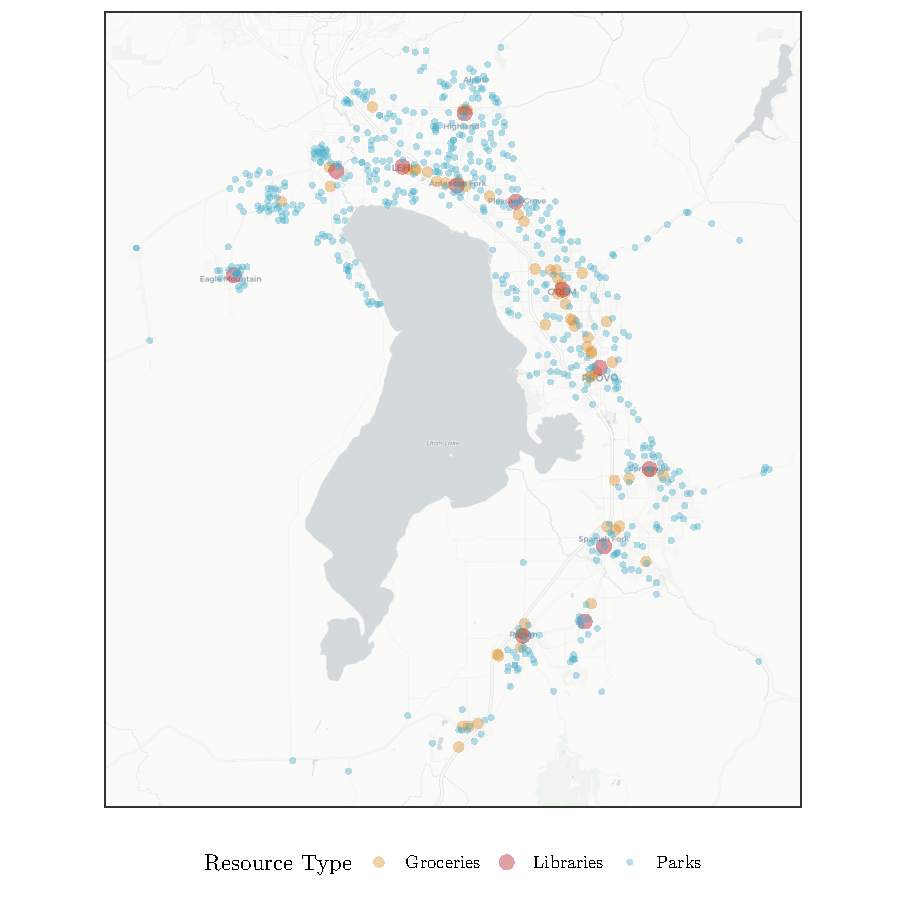
\includegraphics{Community_Resources_files/figure-latex/utco-map-1} 

}

\caption{Location of community resources in Utah County}\label{fig:utco-map}
\end{figure}

\hypertarget{resource-data}{%
\subsubsection{Resource Data}\label{resource-data}}

Figure \ref{fig:utco-map} shows the locations of three types of
community resources in Utah County: parks, grocery stores, and libraries.
For each resource, an initial list of resources and elementary attributes was
obtained by executing a relevant query to OpenStreetMap (OSM).

Public parks and their attributes retrieved from OSM were verified and
corrected using aerial imagery and some site visits. The attributes included
the size of the park in acres, whether the park includes a playground, and
whether the park includes facilities for volleyball, basketball, and tennis.
The constructed dataset includes 582 attributed parks.

Grocery stores were retrieved from OSM and validated using internet resources and
site visits. The complete Nutritional Environment Measures Survey (NEMS-S) \citep{glanz2007}
was collected for each store, but this preliminary analysis only includes
cursory information on the stores including whether the store is a convenience store
or some other non-traditional grocery, whether the store includes a pharmacy or
other non-food merchandise, and the number of registers as a measure of the
store's size. The constructed dataset includes 58 stores.

Libraries were retrieved from OSM, and validated using library websites and
some site visits. The initial query returned university libraries and other
specialty resources; though some of these libraries are open to those outside
the university community, these were removed so that the resource list only
includes libraries generally catering to the general public. The amenities
available include whether the library offers additional classes and programs,
and whether the library includes genealogical or family history resources. The
square footage of the library was estimated from online mapping services.
Other variables discussed in the literature such as the availability of computers
and public wi-fi networks were present in every library and therefore cannot
be included in the destination utility equations.

\hypertarget{mobile-device-data}{%
\subsubsection{Mobile Device Data}\label{mobile-device-data}}

\citet{alamedaparks} present a method for estimating destination choice models from
such data, which we repeat in this study. We provided a set of geometric
polygons for each park, grocery store, and library to StreetLight Data, Inc., a
commercial aggregator. StreetLight Data in turn provided data on the number of
mobile devices observed in each polygon grouped by the inferred residence block
group of of those devices during summer and fall 2019.
We then created a simulated destination choice estimation dataset for each
community resource by sampling 10,000 block group - resource ``trips'' from the
StreetLight dataset. This created a ``chosen'' alternative; we then sampled ten additional
resources at random (each simulated trip was paired with a different sample) to
serve as the non-chosen alternatives. Random sampling of alternatives is a
common practice that results in unbiased estimates, though the standard errors
of the estimates might be larger than could be obtained through a more carefully
designed sampling scheme \citep{train2009}.

\hypertarget{travel-times}{%
\subsubsection{Travel Times}\label{travel-times}}

Once the choice, alternatives, and attributes of the alternatives have been
defined, the last element of the choice utility is the travel impedance between
each block group and each resource. Using the \texttt{r5r} R interface \citep{r5r} to the R5
routing algorithm, we estimated the highway drive travel time, the walking
route time, and the transit travel time for trips departing on April 26,
2022 at 8 AM. The time and date are most relevant for the transit path builder
in R5, which uses detailed transit path information stored in the
Utah Transit Authority GTFS feed file for Spring and Summer 2022. The transit path contains
separate measures of the total travel time, the time in the transit vehicle,
transfer time, and access / egress time, allowing us full use of the
mode choice utility equations and resulting logsum described in Equation \eqref{eq:mcls}.
We limited valid paths to those involving less than 10 km of walking and
2 hours of total travel time.

For groceries and libraries, we queried the shortest time path on each
mode from the population-weighted block group centroid to the centroid of the grocery
store or library polygon. Because some parks in the dataset can be relatively
large and the centroid might be far from the park access or use point, we instead
sampled points along the boundary of the park polygon, and queried the shortest
time path by each mode to the nearest boundary point.

\hypertarget{results}{%
\section{Results}\label{results}}

\hypertarget{destination-choice-models}{%
\subsection{Destination Choice Models}\label{destination-choice-models}}

Using the simulated trip choices assembled from the location-based services data,
we estimate destination choice models with the \texttt{mlogit} package for
R \citep{R, mlogit}.

\begin{table}

\caption{\label{tab:park-models}Park Destination Choice Utilities}
\centering
\resizebox{\linewidth}{!}{
\begin{tabular}[t]{lccccc}
\toprule
  & Car & MCLS & Attributes & All - Car & All - Logsum\\
\midrule
Drive time & -0.286(-93.013)** &  &  & -0.267(-67.263)** & \\
Mode Choice Logsum &  & 10.203(93.013)** &  &  & 9.547(67.263)**\\
log(Acres) &  &  & 1.317(77.828)** & 1.307(45.585)** & 1.307(45.582)**\\
Playground &  &  & 4.574(34.228)** & 4.467(30.248)** & 4.466(30.247)**\\
Volleyball &  &  & -0.344(-8.989)** & -0.555(-9.379)** & -0.555(-9.379)**\\
Basketball &  &  & -0.665(-15.643)** & -0.508(-7.024)** & -0.508(-7.024)**\\
Tennis &  &  & -0.566(-13.515)** & -0.881(-14.706)** & -0.881(-14.708)**\\
\midrule
Num.Obs. & 9,119 & 9,119 & 9,119 & 9,119 & 9,119\\
Log Likelihood & -8945.6 & -8944.8 & -11954.7 & -4603.5 & -4603.2\\
McFadden Rho-Sq & 0.591 & 0.591 & 0.453 & 0.789 & 0.789\\
\bottomrule
\multicolumn{6}{l}{\rule{0pt}{1em}t-statistics in parentheses. * p $<$ 0.5, ** p $<$ 0.1}\\
\end{tabular}}
\end{table}

Table \ref{tab:park-models} presents the model estimation results for
five different specifications of park destination choice. The ``Car'' model
includes only the network travel time by car as a predictor of park choice;
the ``MCLS'' model similarly contains only the mode choice logsum as an
impedance term. The signs on the coefficient indicate that people are more
likely to choose parks with lower car distance or higher multi-modal access, all
else equal. The ``Attributes'' model includes only information on the park attributes
including size and amenities. On balance, people appear attracted to larger parks
and parks with playgrounds, while somewhat deterred by various sports facilities.
The ``All'' models include both the relevant travel impedance term as well as
destination attributes.

For most block group-park pairs, the transit and walk travel disutilities
are sufficiently high that choosing these travel modes is unlikely. As a
result, the mode choice logsum is highly collinear with the car travel time.
Nevertheless, there are small differences differences between the models
with the different impedance terms. Using a non-nested likelihood statistic
test presented by \citet{horowitz1987}, we cannot reject the null hypothesis that the two
``All'' models have equivalent likelihood (\(p\)-value of 0.195), and therefore
cannot infer that the mode choice logsum is a marginally better estimator of
park choice than the vehicle travel time alone.

\begin{table}

\caption{\label{tab:grocery-models}Grocery Destination Choice Utilities}
\centering
\resizebox{\linewidth}{!}{
\begin{tabular}[t]{lcccccc}
\toprule
  & Car & MCLS & Attributes & Size & All - Car & All - Logsum\\
\midrule
Drive time & -0.251(-94.328)** &  &  &  & -0.270(-82.644)** & \\
Mode Choice Logsum &  & 8.972(94.329)** &  &  &  & 9.643(82.645)**\\
Convenience Store &  &  & -2.231(-12.434)** & -1.520(-8.412)** & -1.343(-6.987)** & -1.343(-6.987)**\\
Other non-standard &  &  & -2.224(-15.998)** & -1.618(-11.535)** & -1.418(-9.430)** & -1.418(-9.429)**\\
Has pharmacy &  &  & 0.603(20.852)** & 0.359(10.659)** & 0.330(7.848)** & 0.330(7.850)**\\
Ethnic market &  &  & -1.639(-18.212)** & -0.976(-10.569)** & -0.887(-9.080)** & -0.887(-9.082)**\\
Has other merchandise &  &  & 1.495(51.750)** & 0.791(21.345)** & 0.909(19.288)** & 0.909(19.291)**\\
Number of registers &  &  &  & 0.071(44.314)** & 0.087(40.073)** & 0.087(40.074)**\\
Number of self-checkout &  &  &  & 0.026(13.475)** & 0.020(8.207)** & 0.020(8.206)**\\
\midrule
Num.Obs. & 10,000 & 10,000 & 10,000 & 10,000 & 10,000 & 10,000\\
Log Likelihood & -14256.7 & -14257.0 & -20199.6 & -19031.4 & -10542.9 & -10542.9\\
McFadden Rho-Sq & 0.405 & 0.405 & 0.158 & 0.206 & 0.560 & 0.560\\
\bottomrule
\multicolumn{7}{l}{\rule{0pt}{1em}t-statistics in parentheses. * p $<$ 0.5, ** p $<$ 0.1}\\
\end{tabular}}
\end{table}

Table \ref{tab:grocery-models} presents the model estimation results for the grocery
store models. As with the parks models in Table \ref{tab:park-models}, the
most predictive model contains both a travel impedance term and attributes of
the destination grocery store. The number of registers suggests that people
prefer larger stores, all else equal; ethnic markets, convenience stores, and other
facilities are less preferred while stores with pharmacies and other merchandise
(clothes, home goods, etc.) attract visitors. The ratio of the drive time and
convenience store coefficients suggests that on average, people are willing to
drive 4.97 minutes to reach a store that is not a convenience store.
In terms of the travel impedance, there is again not a sufficiently large gap in the
model likelihoods to reject that the mode choice logsum and the drive
time are equivalent predictors of grocery store choice.

\begin{table}

\caption{\label{tab:library-models}Library Destination Choice Utilities}
\centering
\resizebox{\linewidth}{!}{
\begin{tabular}[t]{lccccc}
\toprule
  & Car & MCLS & Attributes & All - Car & All - Logsum\\
\midrule
Drive time & -0.303(-91.448)** &  &  & -0.313(-72.838)** & \\
Mode Choice Logsum &  & 10.814(91.447)** &  &  & 11.195(72.836)**\\
Offers Classes &  &  & -0.471(-11.662)** & -0.819(-12.050)** & -0.819(-12.051)**\\
Genealogy Resources &  &  & -0.831(-30.213)** & -0.867(-20.844)** & -0.867(-20.840)**\\
log(Square Footage) &  &  & 1.114(79.831)** & 1.219(44.555)** & 1.219(44.552)**\\
\midrule
Num.Obs. & 10,000 & 10,000 & 10,000 & 10,000 & 10,000\\
Log Likelihood & -11198.0 & -11197.5 & -17667.4 & -9389.7 & -9389.6\\
McFadden Rho-Sq & 0.533 & 0.533 & 0.263 & 0.608 & 0.608\\
\bottomrule
\multicolumn{6}{l}{\rule{0pt}{1em}t-statistics in parentheses. * p $<$ 0.5, ** p $<$ 0.1}\\
\end{tabular}}
\end{table}

Table \ref{tab:library-models} presents the model estimation results for the
library destination choice models. As with parks and grocery stores, both
travel impedance and destination attributes are significant predictors of
library choice. The strength of the attributes vector is somewhat surprising,
because virtually all libraries in the data set offer the same set of basic amenities
other than the size of the facility. Further,\\
each municipality in Utah County operates its own library rather than
having a system of interconnected library branches as might be typical in
larger cities or other regions. As with grocery stores and parks, there is no significant difference
between the prediction power of the mode choice logsum versus the car travel
time.

\hypertarget{accessibilities}{%
\subsection{Accessibilities}\label{accessibilities}}

Using the results of the ``All - Logsum'' models estimated for each community resource
in the last section, we calculate the total utility-based accessibility measure
for each block group in Utah County. For comparison to a more traditional measure,
we also created buffer-based accessibility terms where a block group has
``access'' to a grocery store if there is one within a 5-minute drive, a
park if there is one within a five-minute walk, and a library if there is one within
a ten-minute drive.

\begin{figure}
\centering
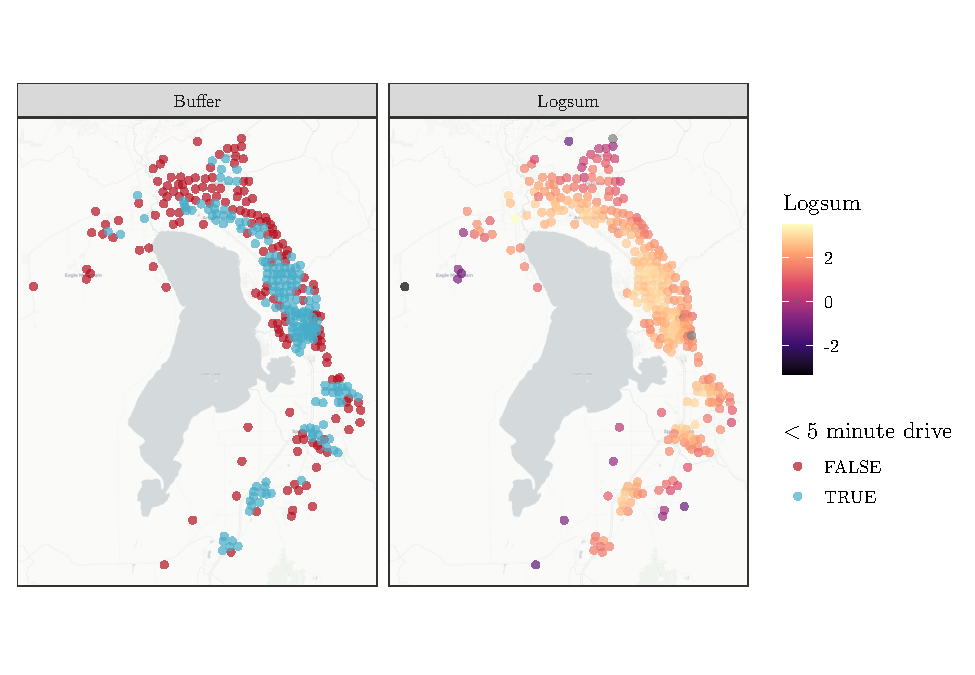
\includegraphics{Community_Resources_files/figure-latex/access-map-1.pdf}
\caption{\label{fig:access-map}Spatial comparison of grocery access buffer versus logsum.}
\end{figure}

Figure \ref{fig:access-map} spatially presents the difference between the
buffer-based measure and the logsum-based measure. The two measures largely
show the same basic shape: block groups along the spine of the county tend
to have binary access in the buffer and also have a higher logsum value. The
difference is at the margins, where the discontinuity of the buffer measure
is replaced by a smoother access surface, more spatially reflective of what
people are likely to experience.

\begin{figure}
\centering
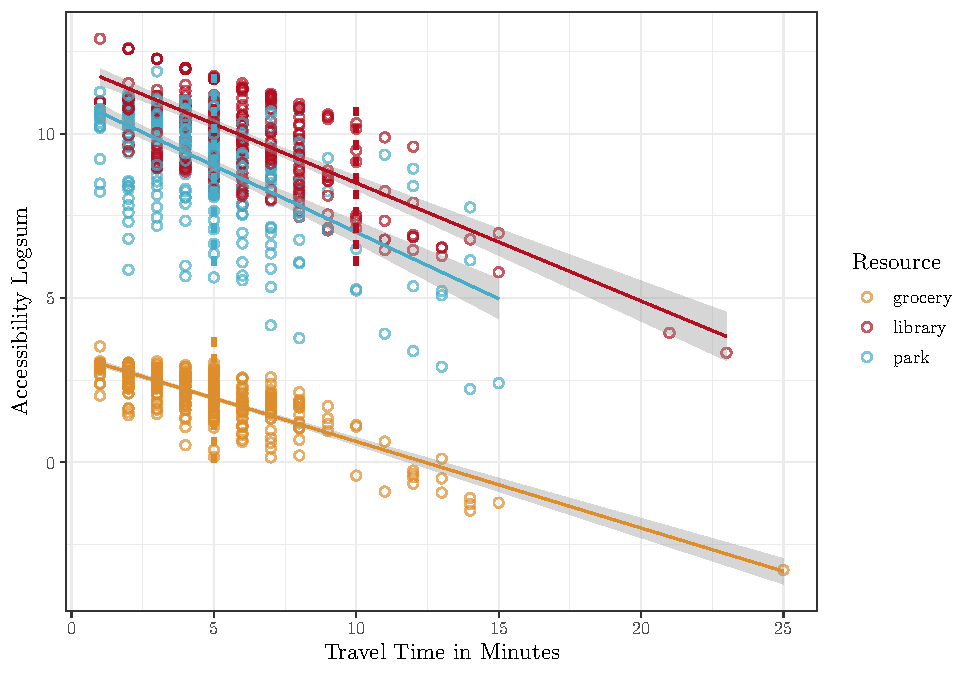
\includegraphics{Community_Resources_files/figure-latex/access-plot-1.pdf}
\caption{\label{fig:access-plot}Relationship between travel time, and logsum access value for block groups in Utah County. Travel-time based buffers shown as dashed lines.}
\end{figure}

The potential for the buffer measure to oversimplify the accessiblity problem is further
illustrated in
Figure \ref{fig:access-plot}. This figure shows the utility-based accessibility
logsum calculated using the mode choice logsum as an impedance term against the
travel time in minutes (drive time for grocery stores and libraries; walk time
for parks), for block groups in the study region. It is clear that for all three
land uses,
lower travel time is significantly correlated with higher accessibility.
But for block groups with with equivalent travel time to a particular community
resource, the accessibility logsum value
varies substantially. Even for block groups along the buffer --- where a small change
in travel time might place a block within or without the buffer --- the variance
in accessibility logsum appears to be almost as large as the variance
in the travel time. This variance in accessiblity logsum might be due to a
travel time differential between drive, walk, and transit modes captured in the
mode choice logsum, or it could also be because the resources available near the
set of block groups have substantial variance in their amenities. Being near a
single poor-quality grocery store is not the same thing as being near multiple
high-quality groceries, and the logsum value can capture this variance in its
construction.

\hypertarget{spatial-distribution}{%
\subsection{Spatial Distribution}\label{spatial-distribution}}

In this analysis,
we estimate that 18,750 households live in block groups outside the
boundary of all three resource buffers: 10-minute drive for a library, 5-minute drive for
a grocery store, and 5-minute walk for a park. Of these, 1,648 make less
than \$35,000 per year.
At the same time, only 33,814 households
live in block groups that are beneath the regional mean utility-based access to
all three resources; that is, they have less-than the regional average access to
grocery stores, and to libraries, and to parks. Of these households, 3,073
are similarly low-income. Perhaps more importantly, the overlap between the households
in \emph{both} groups is not very high: only 9,405 households live
in block groups with low access determined by both buffers and by accessibility
logsum, 739 of which are low-income households.

\hypertarget{discussion}{%
\section{Discussion}\label{discussion}}

The results presented in the previous section suggest that professionals and
academics must understand the implications of accessibility definitions when
conducting spatial analysis of community resources. This study does not attempt
to correlate the accessibility measure it presents with measures of nutrition,
health, or numerous other potential covariates. But it is not difficult to forsee
how the results of such an analysis could change substantially based on whether a
binary distance-based or utility-based definition is used. Further, the lack of
spatial agreement on which people in the community have access or do not have access
implies that policy interventions constructed based on distance alone may target
neighborhoods that actually have good access from a more holistic perspective.

Surely there are limitations to the specific methods developed in this study.
The location-based services data
reveals the likely home location of devices observed within a geographic
polygon, within some measurement error. It cannot tell us whether the device
holder actually accomplished the assumed activity; that is, there may be a
reason why a device was observed near a library even though the person did not
actually patronize the library. Additionally, the method we use to compile the
estimation dataset presumes that the choice to make a trip to the community
resource has already been made. Though it can suggest how the accessibility of a
neighborhood to these resource would improve were transportation impedance
decreased or the resources expanded or improved, it cannot tell us how many more
people might take advantage of the resource in that case.

In this research, all simulated trips were grouped into a single pooled model
for analysis. This implies that the effect of amenities and travel impedance on
destination choice is similar for all neighborhoods. A segmented model
where, for example, low-income block groups and high-income block groups were
estimated separately could allow for flexibility in these estimates and reveal
differences in preferences among residents of the different neighborhoods. Some
neighborhoods might show a particular preference for access utilities by
transit, or for specific park amenities. A latent class choice model \citep{walker2002}
would go further in potentially informing which demographic variables are
meaningful in defining possible data segmentation schemes. It may be also be
possible to estimate the models using a synthetic population with statistical
resampling instead of block group-level aggregate demographic measures.

A necessary assumption made when constructing the estimation dataset is that
people experience access from their home neighborhood. This may not always be true;
for instance, people may choose to shop at grocery stores or visit libraries that
are near their workplace, or that are between their homes and some other
frequent destination. Methods to account for access and destination choices
experienced at other points in the day would be a useful and interesting extension.
Similarly, we assumed that the distance between a home and a community resource
was represented by the distance between the block group centroid and the resource.
For some block groups in less dense areas of the county, the error in measured
travel time between the block group centroid and the actual home location might be
larger than the total travel time. It might be possible to simulate home locations
within each block group and use those locations in the travel time calculations.
Alternatively, it might be possible to estimate the model using block group data
as in this study but apply the model at a more fine resolution (e.g.~block) when
investigating accessibilities and conducting policy analyses.

This paper presents preliminary model estimates using plausible destination
choice utility values. Several additional variables might be further explored,
particularly in regards to the grocery resources. The NEMS-S survey is a highly
detailed picture of the offerings of a particular grocery store, including
information on the availability of relatively healthier or fresher foods and
their prices. This study was only able to explore a few key size variables, but
a deeper investigation into grocery store amenities and offerings
preferences --- and how they might influence a collective understanding of
nutrition access more broadly --- is needed.

\hypertarget{conclusions}{%
\section{Conclusions}\label{conclusions}}

This paper developed accessibility-based measures of accessibility to three
types of community resource: parks, grocery stores, and libraries. These metrics
were informed by observing trips to specific facilities in mobile
device data, allowing the measures to incorporate attributes of the resource
as well as attributes of the journey there. The computed measures are
fundamentally different from buffer-based measures more commonly used to
inform spatial policy analysis.

Ultimately, the purpose of any accessibility measure to a community resources
is to enable a subsequent analysis of some metric of well-being. \citet{macfarlane2020}
suggest that a utility-based access to parks measure is more predictive of
physical health outcomes than a buffer-based measure. Is this true for more
community resources? Would using a more subtle or nuanced measure of access to
libraries help in understanding a link between community form and social isolation
or mental health? A key benefit of this method is that it provides a way to
evaluate the benefit of investments in resources against the benefits of investing
in the transportation system. Will a community benefit more from a new grocery store
nearby, or expanded options at an existing grocery store, or from improving bike
or bus connections to that existing store? An examination of this question is
left for future research, but this paper presents a method for how this could be
approached.

% %%%%%%%%%%%%%%%%%%%%%%%%%%%%%%%%%%%%%%%%%%
% %% optional
% \supplementary{The following are available online at www.mdpi.com/link, Figure S1: title, Table S1: title, Video S1: title.}
%
% % Only for the journal Methods and Protocols:
% % If you wish to submit a video article, please do so with any other supplementary material.
% % \supplementary{The following are available at www.mdpi.com/link: Figure S1: title, Table S1: title, Video S1: title. A supporting video article is available at doi: link.}

\vspace{6pt}

%%%%%%%%%%%%%%%%%%%%%%%%%%%%%%%%%%%%%%%%%%
\acknowledgments{Tables and figures in the article are produced using a variety of packages for R \citep{modelsummary, ggspatial}.
The authors are grateful to Brooke Jones, Kaeli Monahan, and Mali Smith for their help in gathering the grocery
store and library information data. Connor Williams gathered the parks data, and Michael Copley assisted with the
StreetLight data.}

%%%%%%%%%%%%%%%%%%%%%%%%%%%%%%%%%%%%%%%%%%
\authorcontributions{G. Macfarlane conceived and designed the experiments. G. Macfarlane and E. Stucki
performed the experiments. A. Redelfs and L. Spruance designed the data collection
efforts. All authors reviewed and edited the paper from an intial draft by G. Macfarlane.}

%%%%%%%%%%%%%%%%%%%%%%%%%%%%%%%%%%%%%%%%%%
\conflictsofinterest{The authors declare no conflicts of interest.}

%%%%%%%%%%%%%%%%%%%%%%%%%%%%%%%%%%%%%%%%%%
%% optional


%%%%%%%%%%%%%%%%%%%%%%%%%%%%%%%%%%%%%%%%%%
% Citations and References in Supplementary files are permitted provided that they also appear in the reference list here.

%=====================================
% References, variant A: internal bibliography
%=====================================
%\reftitle{References}
%\begin{thebibliography}{999}
% Reference 1
%\bibitem[Author1(year)]{ref-journal}
%Author1, T. The title of the cited article. {\em Journal Abbreviation} {\bf 2008}, {\em 10}, 142--149.
% Reference 2
%\bibitem[Author2(year)]{ref-book}
%Author2, L. The title of the cited contribution. In {\em The Book Title}; Editor1, F., Editor2, A., Eds.; Publishing House: City, Country, 2007; pp. 32--58.
%\end{thebibliography}

% The following MDPI journals use author-date citation: Arts, Econometrics, Economies, Genealogy, Humanities, IJFS, JRFM, Laws, Religions, Risks, Social Sciences. For those journals, please follow the formatting guidelines on http://www.mdpi.com/authors/references
% To cite two works by the same author: \citeauthor{ref-journal-1a} (\citeyear{ref-journal-1a}, \citeyear{ref-journal-1b}). This produces: Whittaker (1967, 1975)
% To cite two works by the same author with specific pages: \citeauthor{ref-journal-3a} (\citeyear{ref-journal-3a}, p. 328; \citeyear{ref-journal-3b}, p.475). This produces: Wong (1999, p. 328; 2000, p. 475)

%=====================================
% References, variant B: external bibliography
%=====================================
\reftitle{References}
\externalbibliography{yes}
\bibliography{book.bib}

%%%%%%%%%%%%%%%%%%%%%%%%%%%%%%%%%%%%%%%%%%
%% optional

%% for journal Sci
%\reviewreports{\\
%Reviewer 1 comments and authors’ response\\
%Reviewer 2 comments and authors’ response\\
%Reviewer 3 comments and authors’ response
%}

%%%%%%%%%%%%%%%%%%%%%%%%%%%%%%%%%%%%%%%%%%


\end{document}
